\documentclass[aspectratio=169,11pt]{beamer}
\usepackage[T1]{fontenc}
\usepackage{lmodern}
\usepackage{graphicx}
\usepackage{xcolor}
\usepackage{tikz}
\usetikzlibrary{calc,positioning,arrows.meta}
\graphicspath{{figs/}}
\usefonttheme{professionalfonts}
\setbeamertemplate{navigation symbols}{}
\definecolor{owpaper}{HTML}{FBFAF6}
\definecolor{owink}{HTML}{16242E}
\definecolor{owdeep}{HTML}{0B2E4F}
\definecolor{owblue}{HTML}{1E6FB0}
\definecolor{owteal}{HTML}{0F8C8C}
\definecolor{owochre}{HTML}{D98A2B}
\definecolor{owmuted}{HTML}{5B6B78}
\setbeamercolor{background canvas}{bg=owpaper}
\setbeamercolor{normal text}{fg=owink}
\setbeamercolor{frametitle}{fg=owdeep}
\setbeamercolor{itemize item}{fg=owteal}
\setbeamercolor{itemize subitem}{fg=owochre}
\setbeamercolor{structure}{fg=owblue}
\setbeamerfont{frametitle}{series=\bfseries,size=\Large}
\setbeamertemplate{itemize item}{\small\raise0.5pt\hbox{\textbullet}}
\setbeamertemplate{frametitle}{%
  \vskip6pt\hbox{\color{owochre}\rule[2pt]{16pt}{2.2pt}}\hskip4pt
  \insertframetitle\par\vskip-2pt}
% nested-worlds mark
\newcommand{\owmark}[1][0.5]{\begin{tikzpicture}[scale=#1]
  \draw[owdeep,line width=1.1pt,rounded corners=1pt] (0,0) rectangle (1,1);
  \draw[owblue,line width=1.1pt,rounded corners=1pt] (0.22,0.22) rectangle (0.78,0.78);
  \fill[owteal,rounded corners=0.5pt] (0.40,0.40) rectangle (0.60,0.60);
\end{tikzpicture}}
\setbeamertemplate{footline}{\hbox{}\hfill{\color{owmuted}\tiny\insertframenumber}\hskip8pt\vskip4pt}

\begin{document}
\begin{frame}[plain]
\centering\vfill
{\owmark[1.4]}\par\vskip14pt
{\color{owdeep}\bfseries\LARGE World Models: An Overview and Applications\par}\vskip8pt
{\color{owblue}\large Verified code world models — build, verify, compose, traverse, and serve simulated worlds\par}\vskip18pt
{\color{owink}\normalsize Jim Schwoebel — Quome / OpenWorld\par}\vskip3pt
{\color{owmuted}\small github.com/quome-cloud/openworld\par}
\vfill
\end{frame}

\begin{frame}[plain]\centering\vfill
{\color{owochre}\rule{40pt}{2.5pt}}\par\vskip10pt
{\color{owdeep}\bfseries\Large What is a world model?\par}\vfill\end{frame}
\begin{frame}{The unit of world computing}
\begin{itemize}
  \item A world model predicts the next state given a state and an action
  \item World = symbolic state + discrete actions + a transition rule
  \item One world serves as both ground-truth environment and planning model
  \item Agents are separate policies -- users of a world, not part of it
\end{itemize}
\end{frame}
\begin{frame}{Two species of world models}
\begin{itemize}
  \item Perceptual/generative: neural nets over pixels/latents (Dreamer, Genie, Sora)
  \item Powerful, but data-hungry, compounding, and opaque
  \item Code World Models: the transition is a readable program over symbolic state
  \item Synthesized by an LLM, verified before use, exact and inspectable
  \item Complementary tools, not competitors
\end{itemize}
\end{frame}
\begin{frame}{Why verified code}
\begin{itemize}
  \item Value is exact, fast, auditable execution an agent can call as a tool
  \item Deterministic: no compounding error; learned dynamics decay as (1-e)\textasciicircum{}t
  \item Plain code rolls out \textasciitilde{}47,000x faster than a per-step LLM proxy
  \item The artifact stays a diffable program at every stage
\end{itemize}
\end{frame}
\begin{frame}[plain]\centering\vfill
{\color{owdeep}\bfseries\LARGE Make the model a program, verify the program, and keep the values dialable.\par}\vfill\end{frame}
\begin{frame}{Three results, one substrate}\vfill\begin{columns}[c]\begin{column}{0.323\textwidth}\centering{\color{owdeep}\fontsize{40}{44}\selectfont\bfseries 100}\\[6pt]{\color{owmuted}\small verified worlds authored in minutes}\end{column}\begin{column}{0.323\textwidth}\centering{\color{owdeep}\fontsize{40}{44}\selectfont\bfseries +29 pts}\\[6pt]{\color{owmuted}\small world-time-compute lift (0.5B)}\end{column}\begin{column}{0.323\textwidth}\centering{\color{owochre}\fontsize{40}{44}\selectfont\bfseries 25/25}\\[6pt]{\color{owmuted}\small ARC-AGI-3, source-free}\end{column}\end{columns}\vfill\end{frame}
\begin{frame}[plain]\centering\vfill
{\color{owochre}\rule{40pt}{2.5pt}}\par\vskip10pt
{\color{owdeep}\bfseries\Large The substrate: OpenWorld\par}\vfill\end{frame}
\begin{frame}{One agent authors validated, serveable worlds}
\centering

\includegraphics[width=\linewidth,height=0.48\textheight,keepaspectratio]{world_computer.png}\vskip3pt{\color{owmuted}\footnotesize Benchmarked on cost, latency, and performance; verified code \textasciitilde{}47,000x faster than an LLM\par}
\flushleft \vskip3pt{\footnotesize \begin{itemize}
  \item 100 worlds authored at a median of 2.8 min each
  \item 14,997 steps/s vs 0.32 for the per-step LLM proxy
  \item 100\% validate structurally; 99\% pass a behavioral audit
\end{itemize}}
\end{frame}
\begin{frame}{A code world model, end to end}
\centering

\includegraphics[width=\linewidth,height=0.48\textheight,keepaspectratio]{prototyping_pipeline.png}\vskip3pt{\color{owmuted}\footnotesize Perceive -> world -> emit/act, generated from a real spec so labels cannot drift\par}
\flushleft \vskip3pt{\footnotesize \begin{itemize}
  \item Perceptors turn any-modality inputs into symbolic state
  \item Verified transitions step inside a composite of nested worlds
  \item Objectives (dial-retuned) score; emit/act returns reports and tool-calls
\end{itemize}}
\end{frame}
\begin{frame}{The plan--generate--verify relay}
\begin{itemize}
  \item Declare a world; a generator writes transition(state, action)
  \item Gate 1: parses; Gate 2: sandboxed run respects invariants; Gate 3: a critic
  \item Accepted code is plain, editable source -- failures loop into the next prompt
  \item Composition is verification-preserving: verified pieces => verified whole
\end{itemize}
\end{frame}
\begin{frame}[plain]\centering\vfill
{\color{owochre}\rule{40pt}{2.5pt}}\par\vskip10pt
{\color{owdeep}\bfseries\Large Result I — World computing\par}\vfill\end{frame}
\begin{frame}{Prototyping is minutes-scale (E68)}
\begin{itemize}
  \item 100 world models across 6 regulated sectors from one-line prompts
  \item Median 2.8 min; 100\% validate; 99\% behaviorally executable
  \item Hand-authoring a comparable simulator is a days-to-weeks effort
\end{itemize}
\end{frame}
\begin{frame}{Fidelity and latency (E04, E11)}
\centering
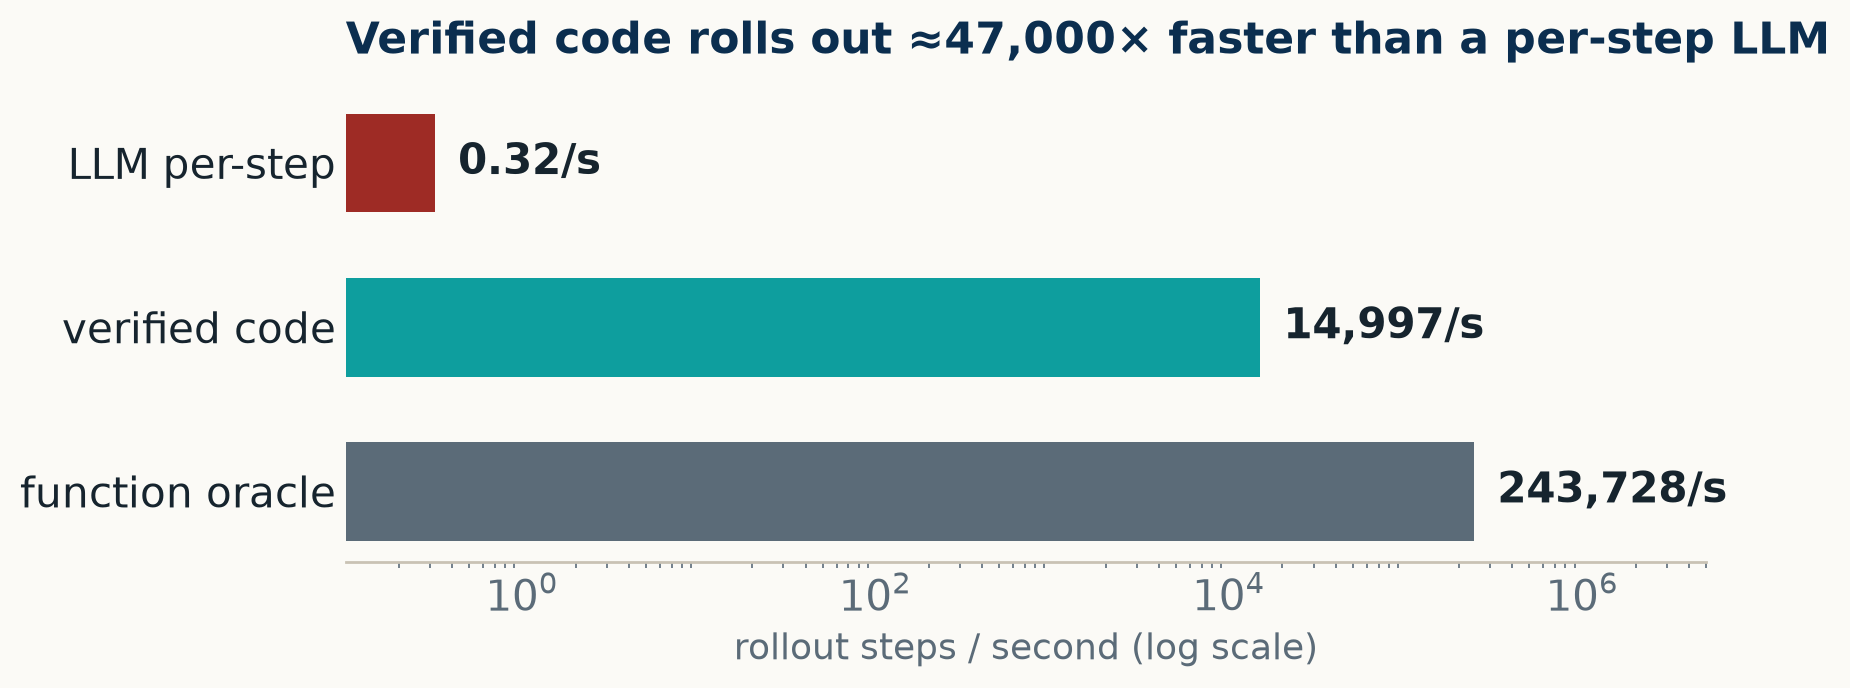
\includegraphics[width=\linewidth,height=0.48\textheight,keepaspectratio]{pres_speed.png}\vskip3pt{\color{owmuted}\footnotesize Exact on 24/24 twenty-step rollouts and 10x OOD probes -- no compounding error\par}
\flushleft \vskip3pt{\footnotesize \begin{itemize}
  \item \textasciitilde{}47,000x faster rollout than a per-step LLM engine
\end{itemize}}
\end{frame}
\begin{frame}{Composition defeats the complexity cliff (E30)}
\centering
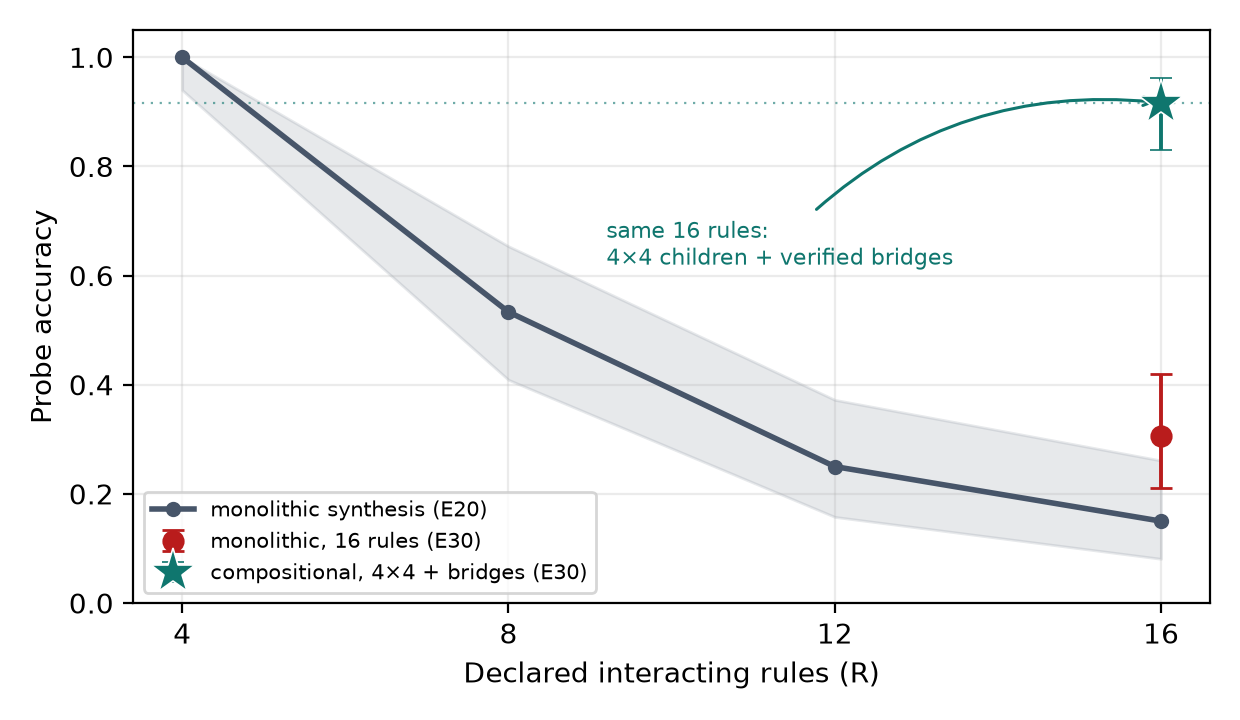
\includegraphics[width=\linewidth,height=0.48\textheight,keepaspectratio]{composition_cliff.png}\vskip3pt{\color{owmuted}\footnotesize 16 rules: monolithic 0.31 vs four 4-rule children + bridges 0.92\par}
\flushleft \vskip3pt{\footnotesize \begin{itemize}
  \item Monolithic synthesis collapses past \textasciitilde{}8 coupled rules
  \item Decomposition returns accuracy to near-R=4 levels
  \item One n-rule problem becomes n small, independently verified ones
\end{itemize}}
\end{frame}
\begin{frame}{Tunable morality: the moral dial (E8)}
\centering

\includegraphics[width=\linewidth,height=0.48\textheight,keepaspectratio]{pareto.png}\vskip3pt{\color{owmuted}\footnotesize Welfare--fairness frontier swept by lambda; values are declared, weighted artifacts\par}
\flushleft \vskip3pt{\footnotesize \begin{itemize}
  \item All sweep points Pareto-optimal; move without retraining
  \item Vetoes and a moral parliament are distinct objects, not weights
  \item Alignment as open specification, managed procedurally
\end{itemize}}
\end{frame}
\begin{frame}[plain]\centering\vfill
{\color{owochre}\rule{40pt}{2.5pt}}\par\vskip10pt
{\color{owdeep}\bfseries\Large Result II — World-time compute\par}\vfill\end{frame}
\begin{frame}{Manufacturing experience}
\begin{itemize}
  \item A verified world is a generator of unlimited exactly-labeled experience
  \item Traverse many worlds of a domain; distill the shared skill
  \item The training-time analogue of test-time compute
  \item Two conditions: verified-label dependence and cross-world transfer
\end{itemize}
\end{frame}
\begin{frame}{Verified code eliminates compounding error}
\centering
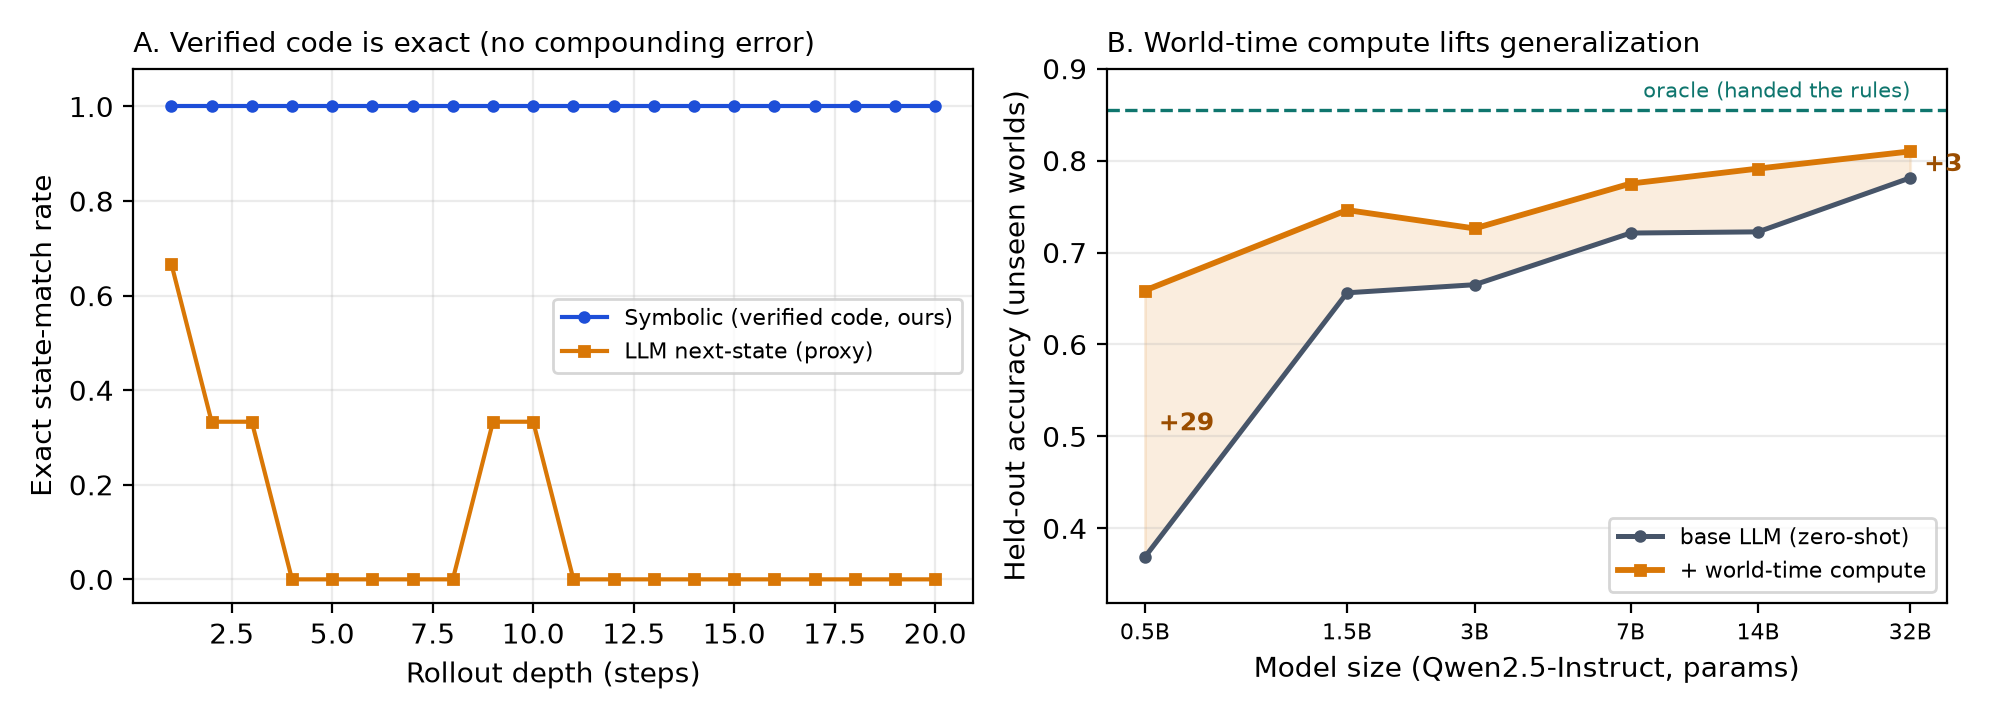
\includegraphics[width=\linewidth,height=0.48\textheight,keepaspectratio]{hero.png}\vskip3pt{\color{owmuted}\footnotesize Code exact at every depth vs LLM diverging \textasciitilde{}step 2.3; fine-tuning on worlds lifts accuracy\par}
\flushleft \vskip3pt{\footnotesize \begin{itemize}
  \item Code matches the oracle exactly across a 20-step rollout
  \item Fine-tuning on 60 verified worlds lifts held-out accuracy
  \item Largest gain for the smallest models: +29 pts at 0.5B
\end{itemize}}
\end{frame}
\begin{frame}{Cross-world transfer scales with \#worlds (E84)}
\centering
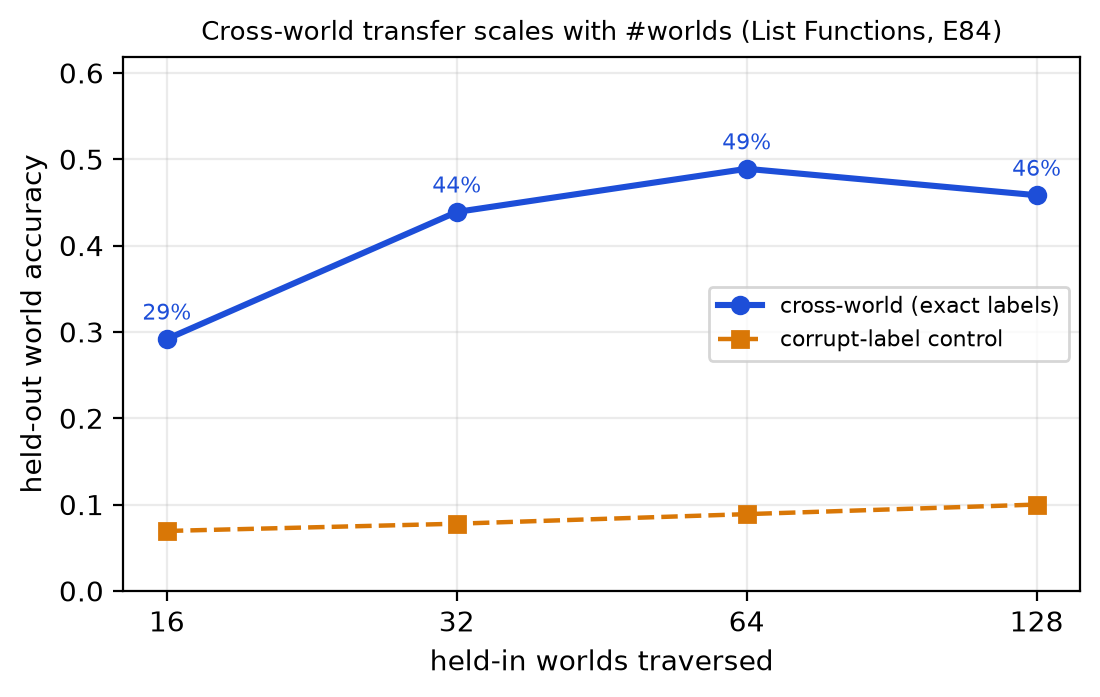
\includegraphics[width=\linewidth,height=0.48\textheight,keepaspectratio]{crossworld_ladder.png}\vskip3pt{\color{owmuted}\footnotesize List Functions held-out accuracy 29\% -> 49\% as the number of verified worlds grows\par}
\flushleft \vskip3pt{\footnotesize \begin{itemize}
  \item One adapter on 128 disjoint worlds generalizes to 60 unseen worlds
  \item Corrupted-label control stays flat -- exact labels are the lever
  \item A real scaling curve on data we did not generate
\end{itemize}}
\end{frame}
\begin{frame}{Across real domains (E80)}
\centering
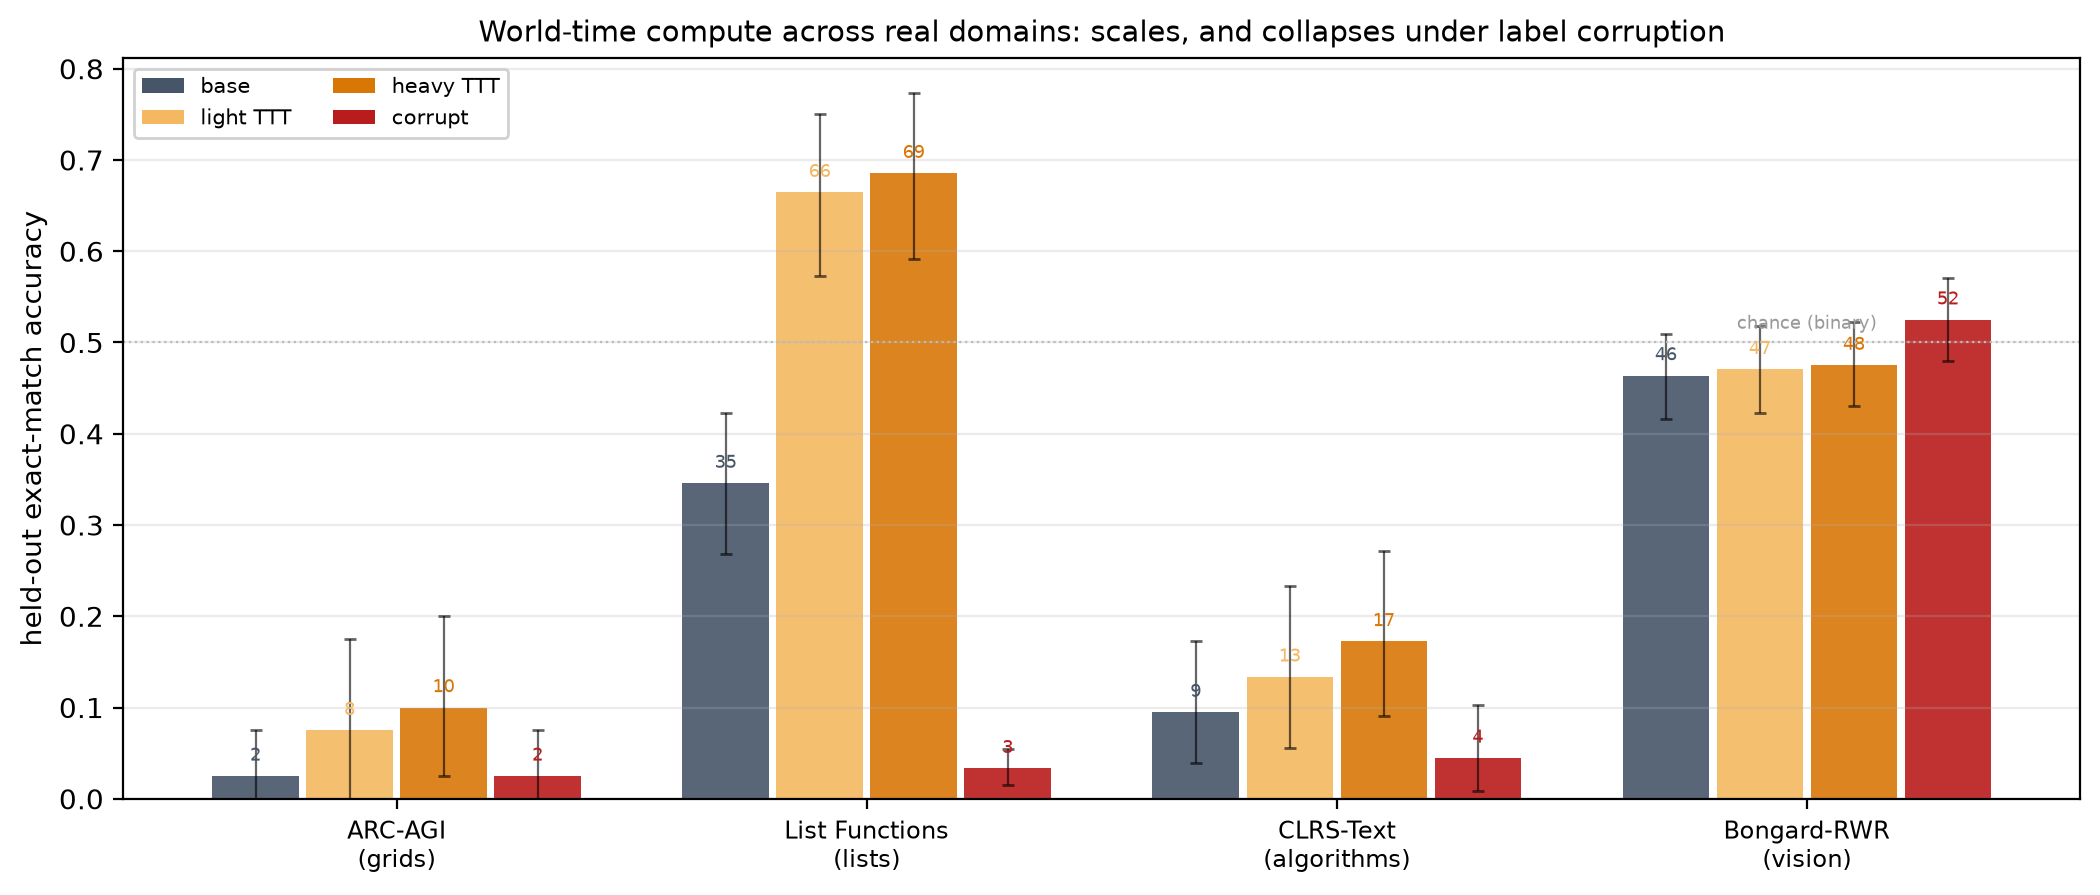
\includegraphics[width=\linewidth,height=0.48\textheight,keepaspectratio]{worldtime_domains.png}\vskip3pt{\color{owmuted}\footnotesize Scales on symbolic domains (List Functions, CLRS, ARC); flat on Bongard vision\par}
\flushleft \vskip3pt{\footnotesize \begin{itemize}
  \item List Functions 35\% -> 69\%; ARC per-world TTT +8 pts
  \item Effect largest for shallow rules, smallest for long traces
  \item Bongard-RWR vision stays at chance -- the perceptual boundary
\end{itemize}}
\end{frame}
\begin{frame}[plain]\centering\vfill
{\color{owochre}\rule{40pt}{2.5pt}}\par\vskip10pt
{\color{owdeep}\bfseries\Large Result III — Solving ARC-AGI-3\par}\vfill\end{frame}
\begin{frame}{A source-free agent that writes its own world model}
\centering
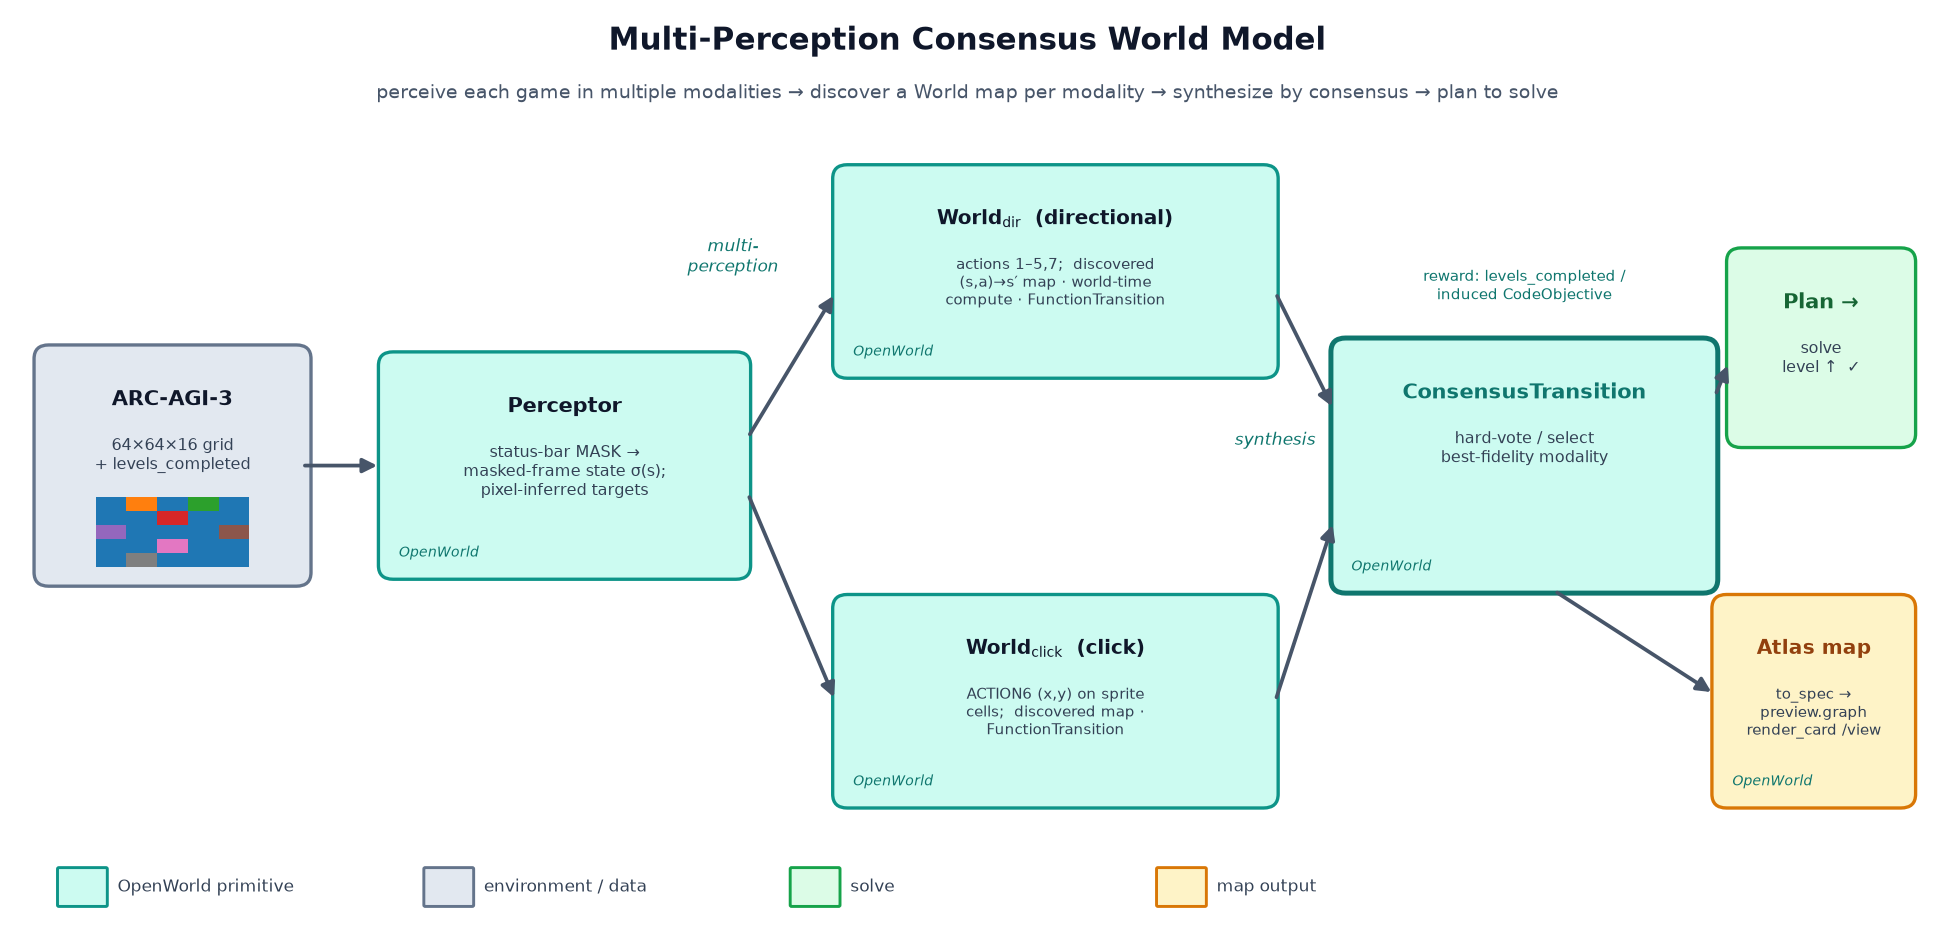
\includegraphics[width=\linewidth,height=0.48\textheight,keepaspectratio]{arc3_architecture.png}\vskip3pt{\color{owmuted}\footnotesize Perceive -> explore -> synthesize verified code -> reason goal -> plan -> replay-verify\par}
\flushleft \vskip3pt{\footnotesize \begin{itemize}
  \item Never reads game code; discovers the rules by acting
  \item Each solve becomes a serveable OpenWorld World
  \item Modeling is exact -- the wall is figuring out the goal
\end{itemize}}
\end{frame}
\begin{frame}{The wall: goal-as-procedure}
\centering

\includegraphics[width=\linewidth,height=0.48\textheight,keepaspectratio]{arc3_goal_as_procedure.png}\vskip3pt{\color{owmuted}\footnotesize A win is an ordered procedure A->B->C, which no single-state score can rank\par}
\flushleft \vskip3pt{\footnotesize \begin{itemize}
  \item Four principled goal-discovery methods solve 0 -- even on a perfect model
  \item State-scoring and blind search cannot rank an ordered protocol
  \item Only a reasoning agent that reasons the win crosses the walls
\end{itemize}}
\end{frame}
\begin{frame}{The first perfect source-free result (model-scaling)}
\centering
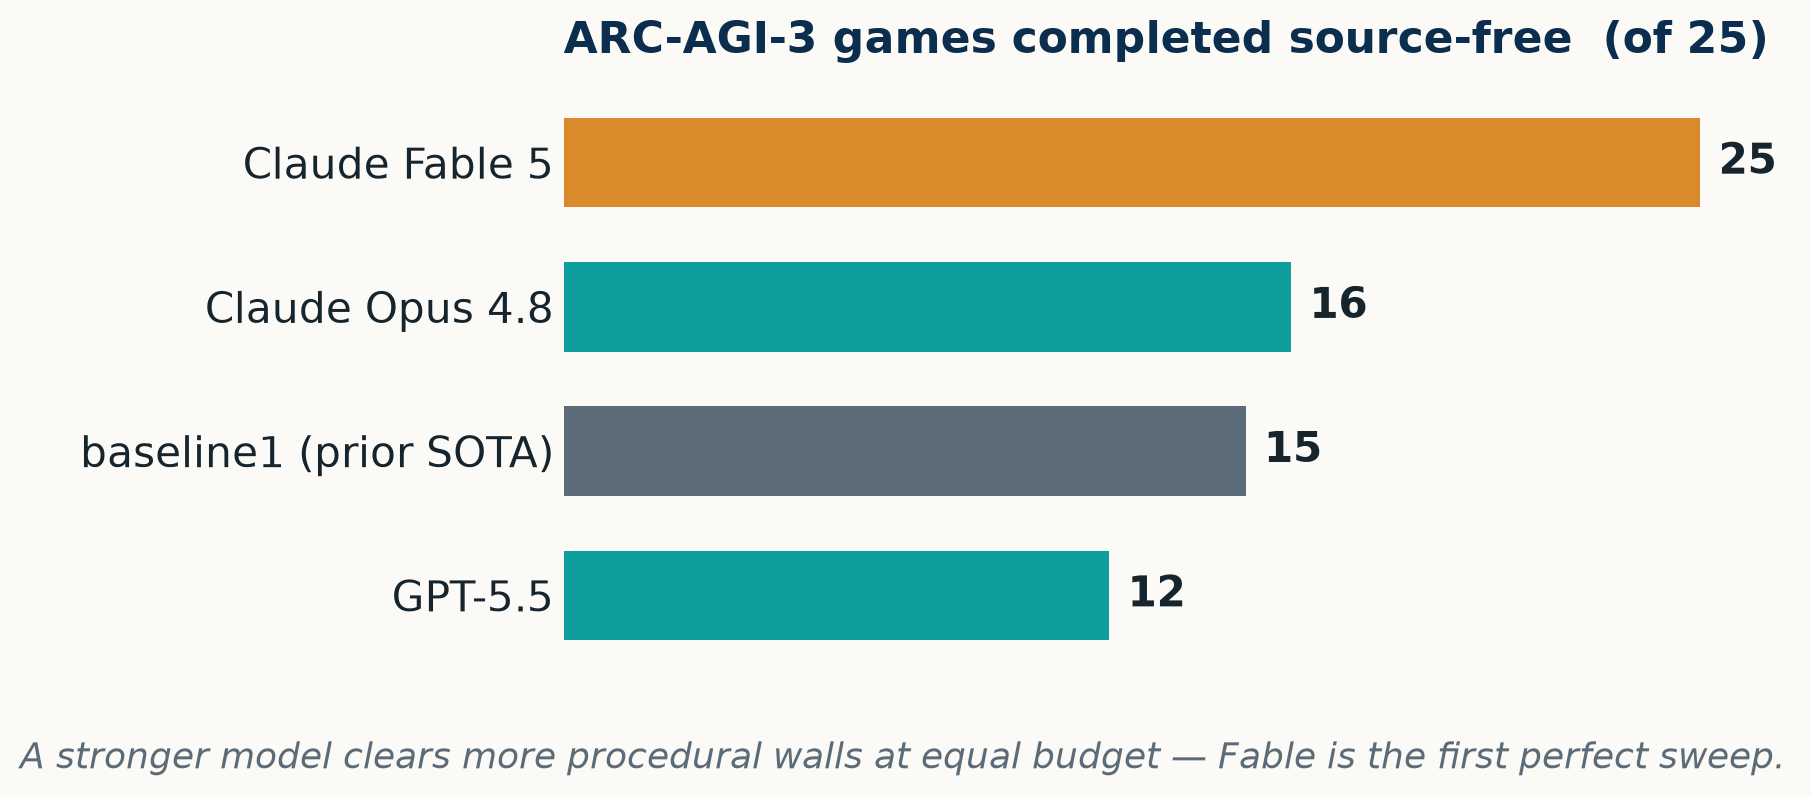
\includegraphics[width=\linewidth,height=0.48\textheight,keepaspectratio]{pres_arc3_scaling.png}\vskip3pt{\color{owmuted}\footnotesize Claude Fable sweeps all 25 games; a stronger model clears more walls at equal budget\par}
\flushleft \vskip3pt{\footnotesize \begin{itemize}
  \item Claude Fable 5: 25/25 games, 183/183 levels -- first perfect result
  \item Opus 4.8: 16/25; GPT-5.5: 12/25; prior best baseline1: 15/25
  \item Capability rises and cost falls: Fable \textasciitilde{}3.5x fewer tokens
\end{itemize}}
\end{frame}
\begin{frame}{The atlas: 25 games, 25 serveable worlds}
\centering

\includegraphics[width=\linewidth,height=0.48\textheight,keepaspectratio]{arc3_maps_gallery.png}\vskip3pt{\color{owmuted}\footnotesize Every source-free solve round-trips to a runnable OpenWorld World\par}
\flushleft \vskip3pt{\footnotesize \begin{itemize}
  \item masked-frame perceptor -> FunctionTransition -> CodeObjective
  \item Serves at openworld serve /view; renders as an atlas card
  \item 25 visibly distinct worlds discovered by acting
\end{itemize}}
\end{frame}
\begin{frame}[plain]\centering\vfill
{\color{owochre}\rule{40pt}{2.5pt}}\par\vskip10pt
{\color{owdeep}\bfseries\Large Applications across domains\par}\vfill\end{frame}
\begin{frame}{Relativity as a verified world model (E47)}
\centering
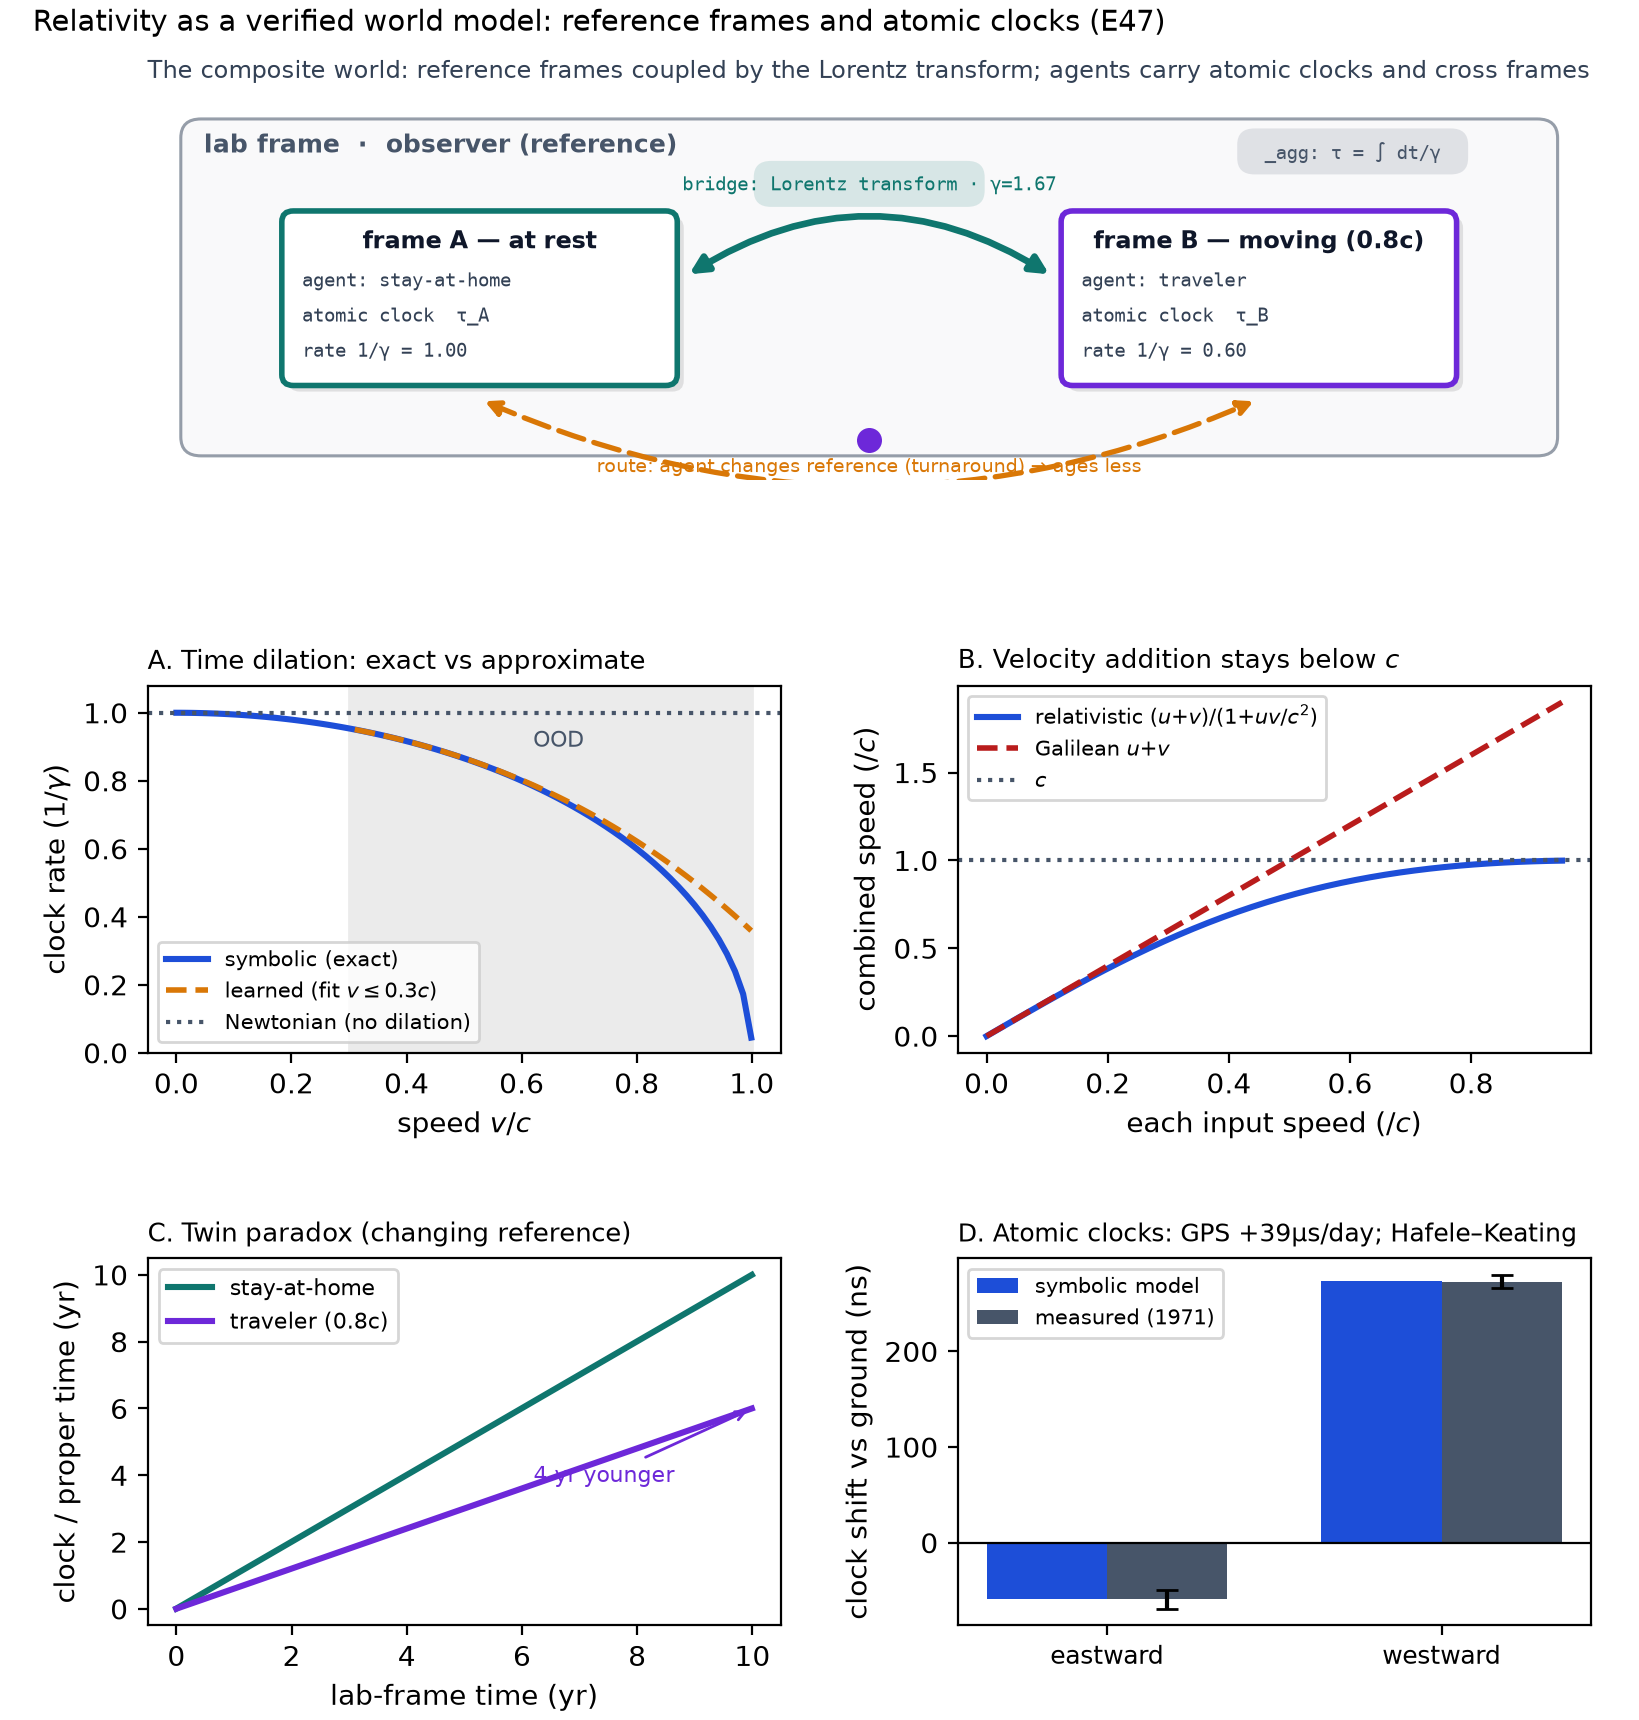
\includegraphics[width=\linewidth,height=0.48\textheight,keepaspectratio]{relativity.png}\vskip3pt{\color{owmuted}\footnotesize GPS correction +38.5 us/day and Hafele--Keating shifts, from declared physics\par}
\flushleft \vskip3pt{\footnotesize \begin{itemize}
  \item Time dilation exact; a low-speed learned fit diverges as v -> c
  \item Declared, verified law where learned video models miss the physics
\end{itemize}}
\end{frame}
\begin{frame}{An emergent economy from composed rules (E44)}
\centering
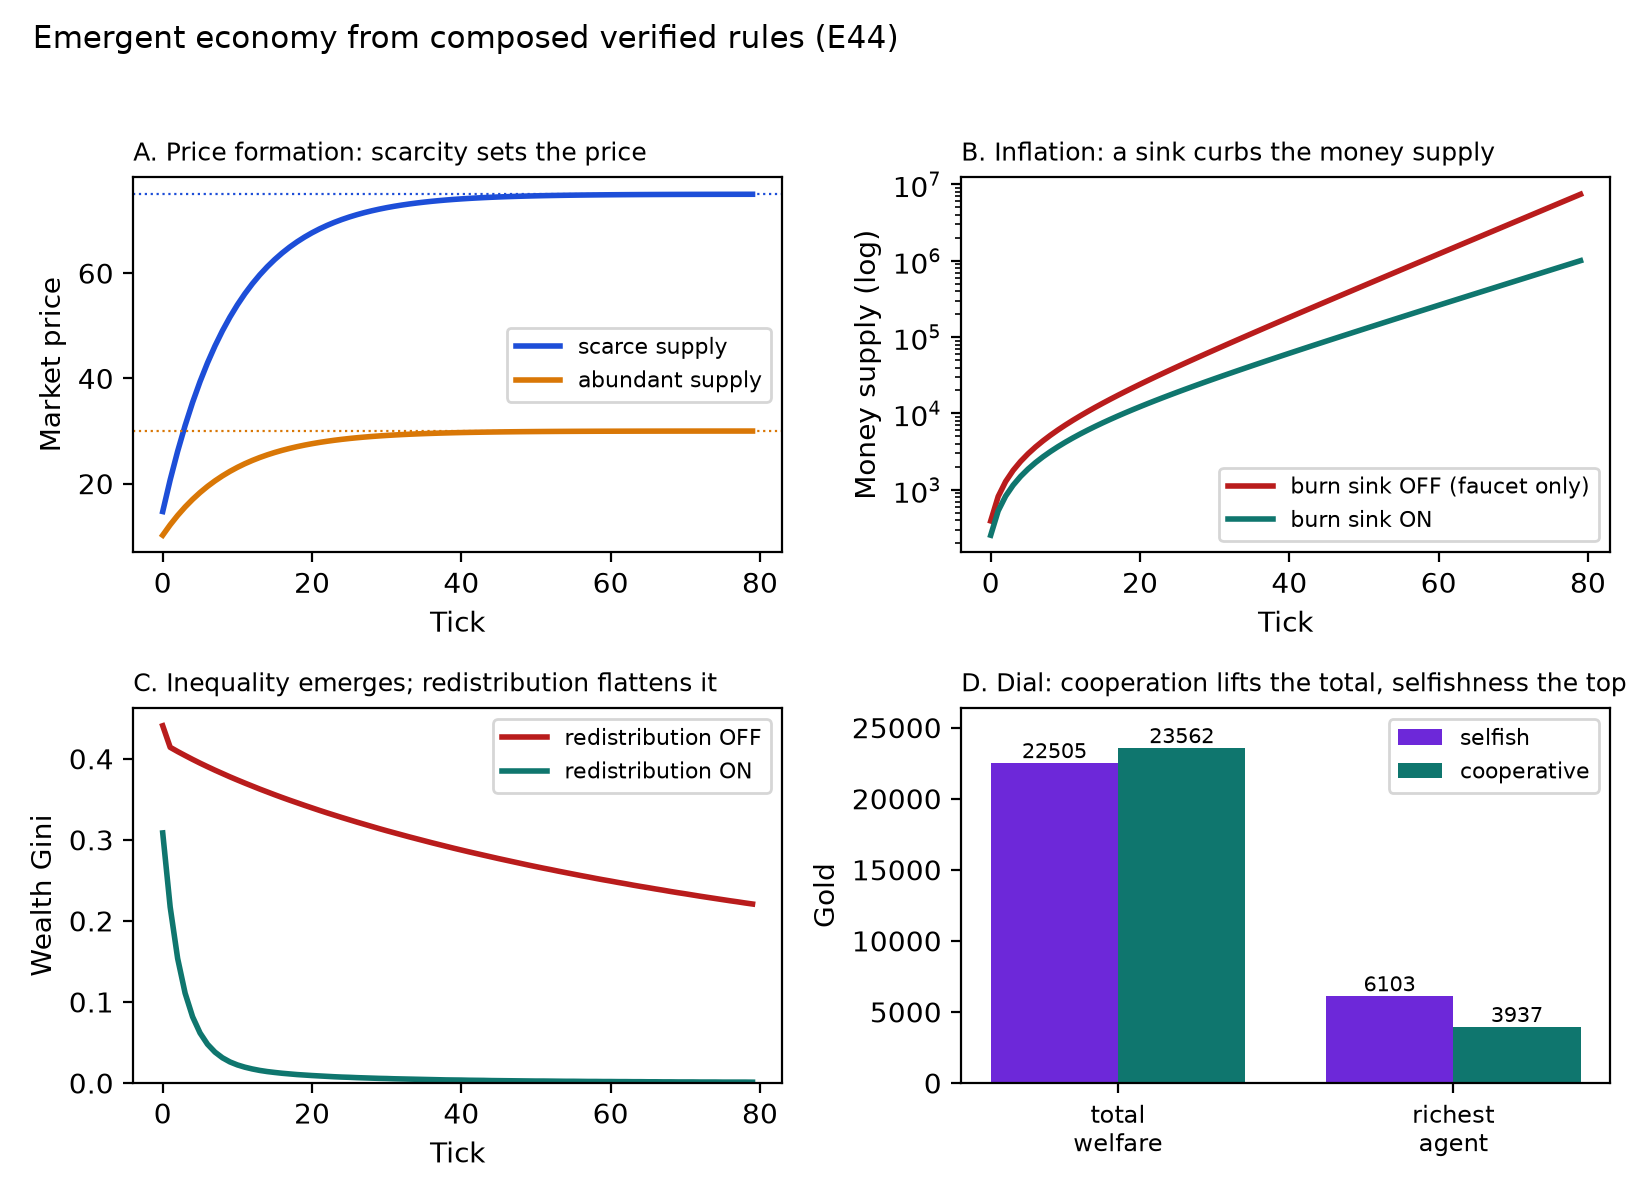
\includegraphics[width=\linewidth,height=0.48\textheight,keepaspectratio]{emergent_economy.png}\vskip3pt{\color{owmuted}\footnotesize 6 agents; Gini 0.22 -> 0.001 with redistribution; books balance exactly every tick\par}
\flushleft \vskip3pt{\footnotesize \begin{itemize}
  \item Macro variables are aggregators derived from verified micro leaves
  \item Each phenomenon isolated by toggling one verified rule
\end{itemize}}
\end{frame}
\begin{frame}{A brain as a world-of-worlds (E58)}
\centering
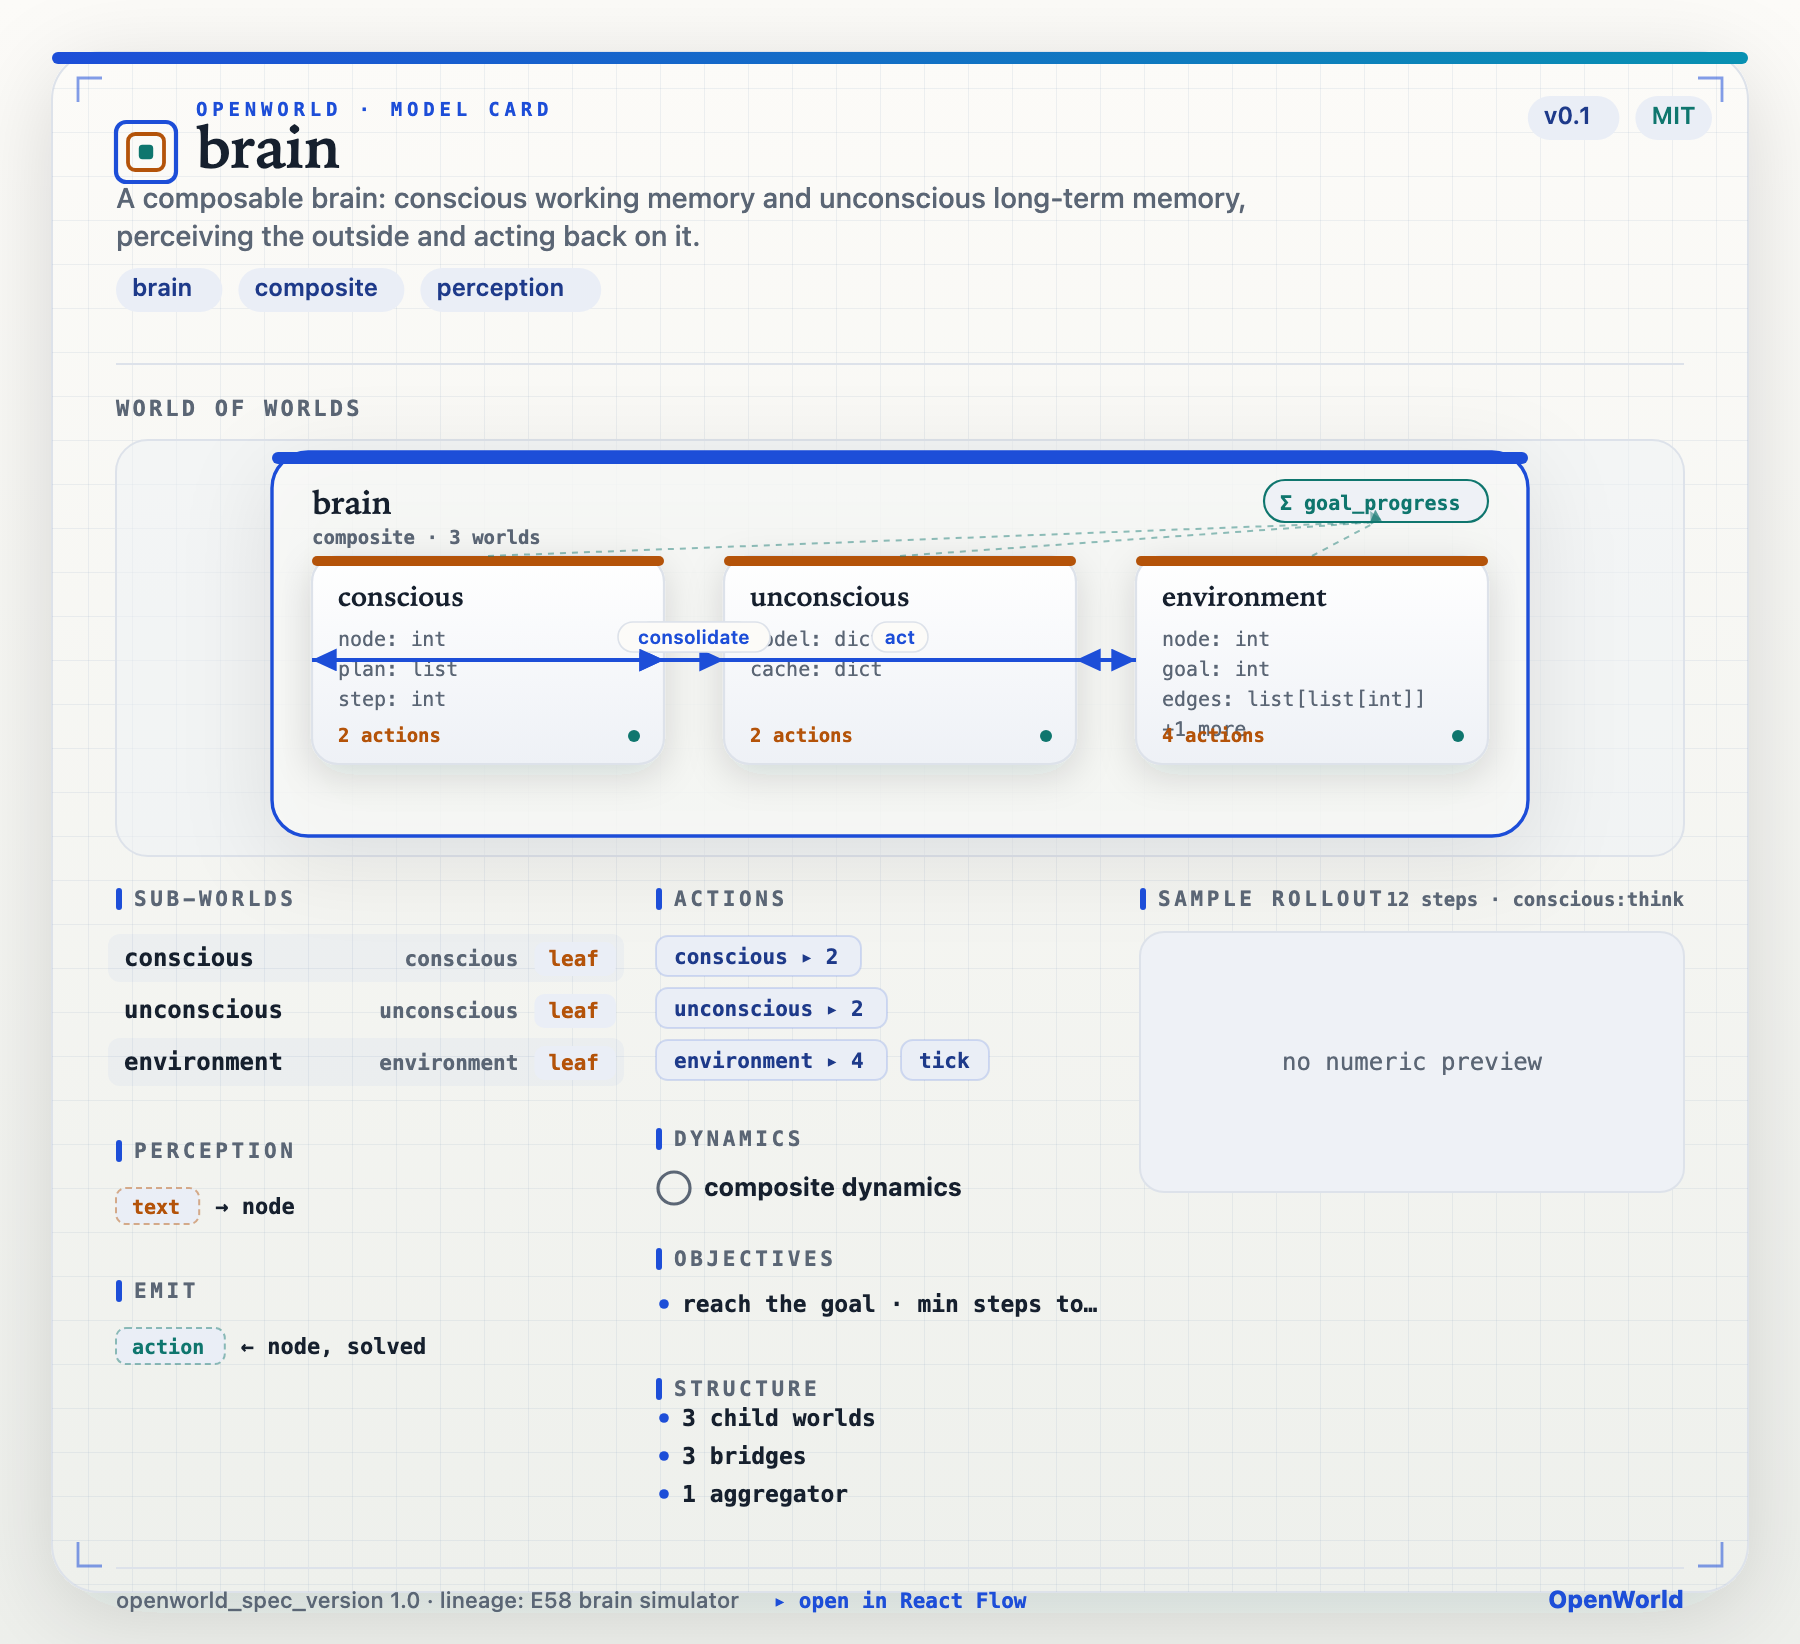
\includegraphics[width=\linewidth,height=0.48\textheight,keepaspectratio]{brain_card.png}\vskip3pt{\color{owmuted}\footnotesize Conscious + unconscious + environment, coupled by retrieve/consolidate/act bridges\par}
\flushleft \vskip3pt{\footnotesize \begin{itemize}
  \item Working memory + content-addressable long-term memory + environment
  \item The whole brain serializes to a spec and round-trips losslessly
\end{itemize}}
\end{frame}
\begin{frame}{Perceive-then-forecast an epidemic (E40)}
\centering

\includegraphics[width=\linewidth,height=0.48\textheight,keepaspectratio]{perception.png}\vskip3pt{\color{owmuted}\footnotesize Perceived world model exact in and out of distribution; the MLP collapses at 10x scale\par}
\flushleft \vskip3pt{\footnotesize \begin{itemize}
  \item Text + photo perceived into S,I,R, then rolled 14 days
  \item Dynamics add zero error -- forecast accuracy equals perception accuracy
\end{itemize}}
\end{frame}
\begin{frame}{A same-day trading world model (E50)}
\centering
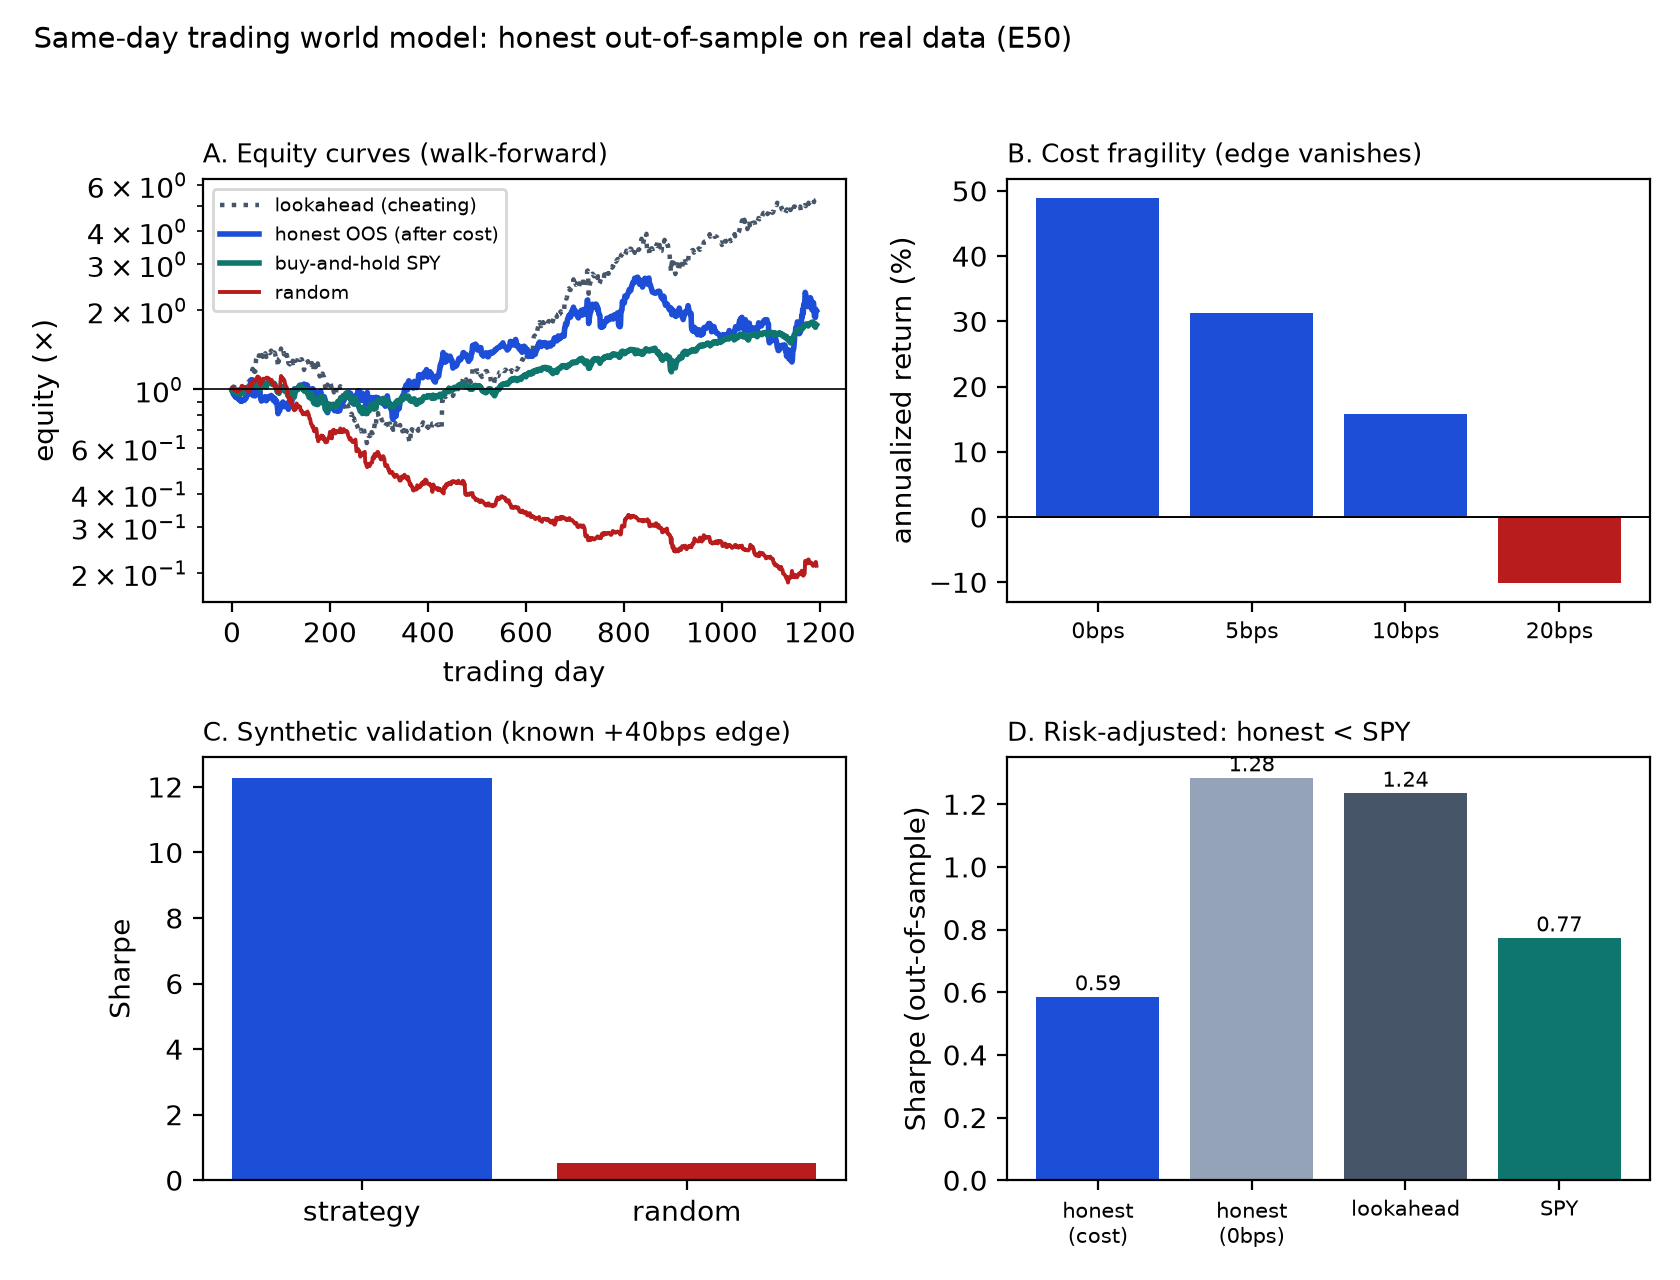
\includegraphics[width=\linewidth,height=0.48\textheight,keepaspectratio]{trading.png}\vskip3pt{\color{owmuted}\footnotesize Real OHLC, walk-forward, after-cost -- rigor and auditability, not alpha\par}
\flushleft \vskip3pt{\footnotesize \begin{itemize}
  \item Recovers a known +40 bps synthetic edge, so a weak real result is real
  \item Honest and cost-fragile: Sharpe 0.59 < SPY 0.77
\end{itemize}}
\end{frame}
\begin{frame}{Portable, auditable world specs and cards (E57)}
\centering
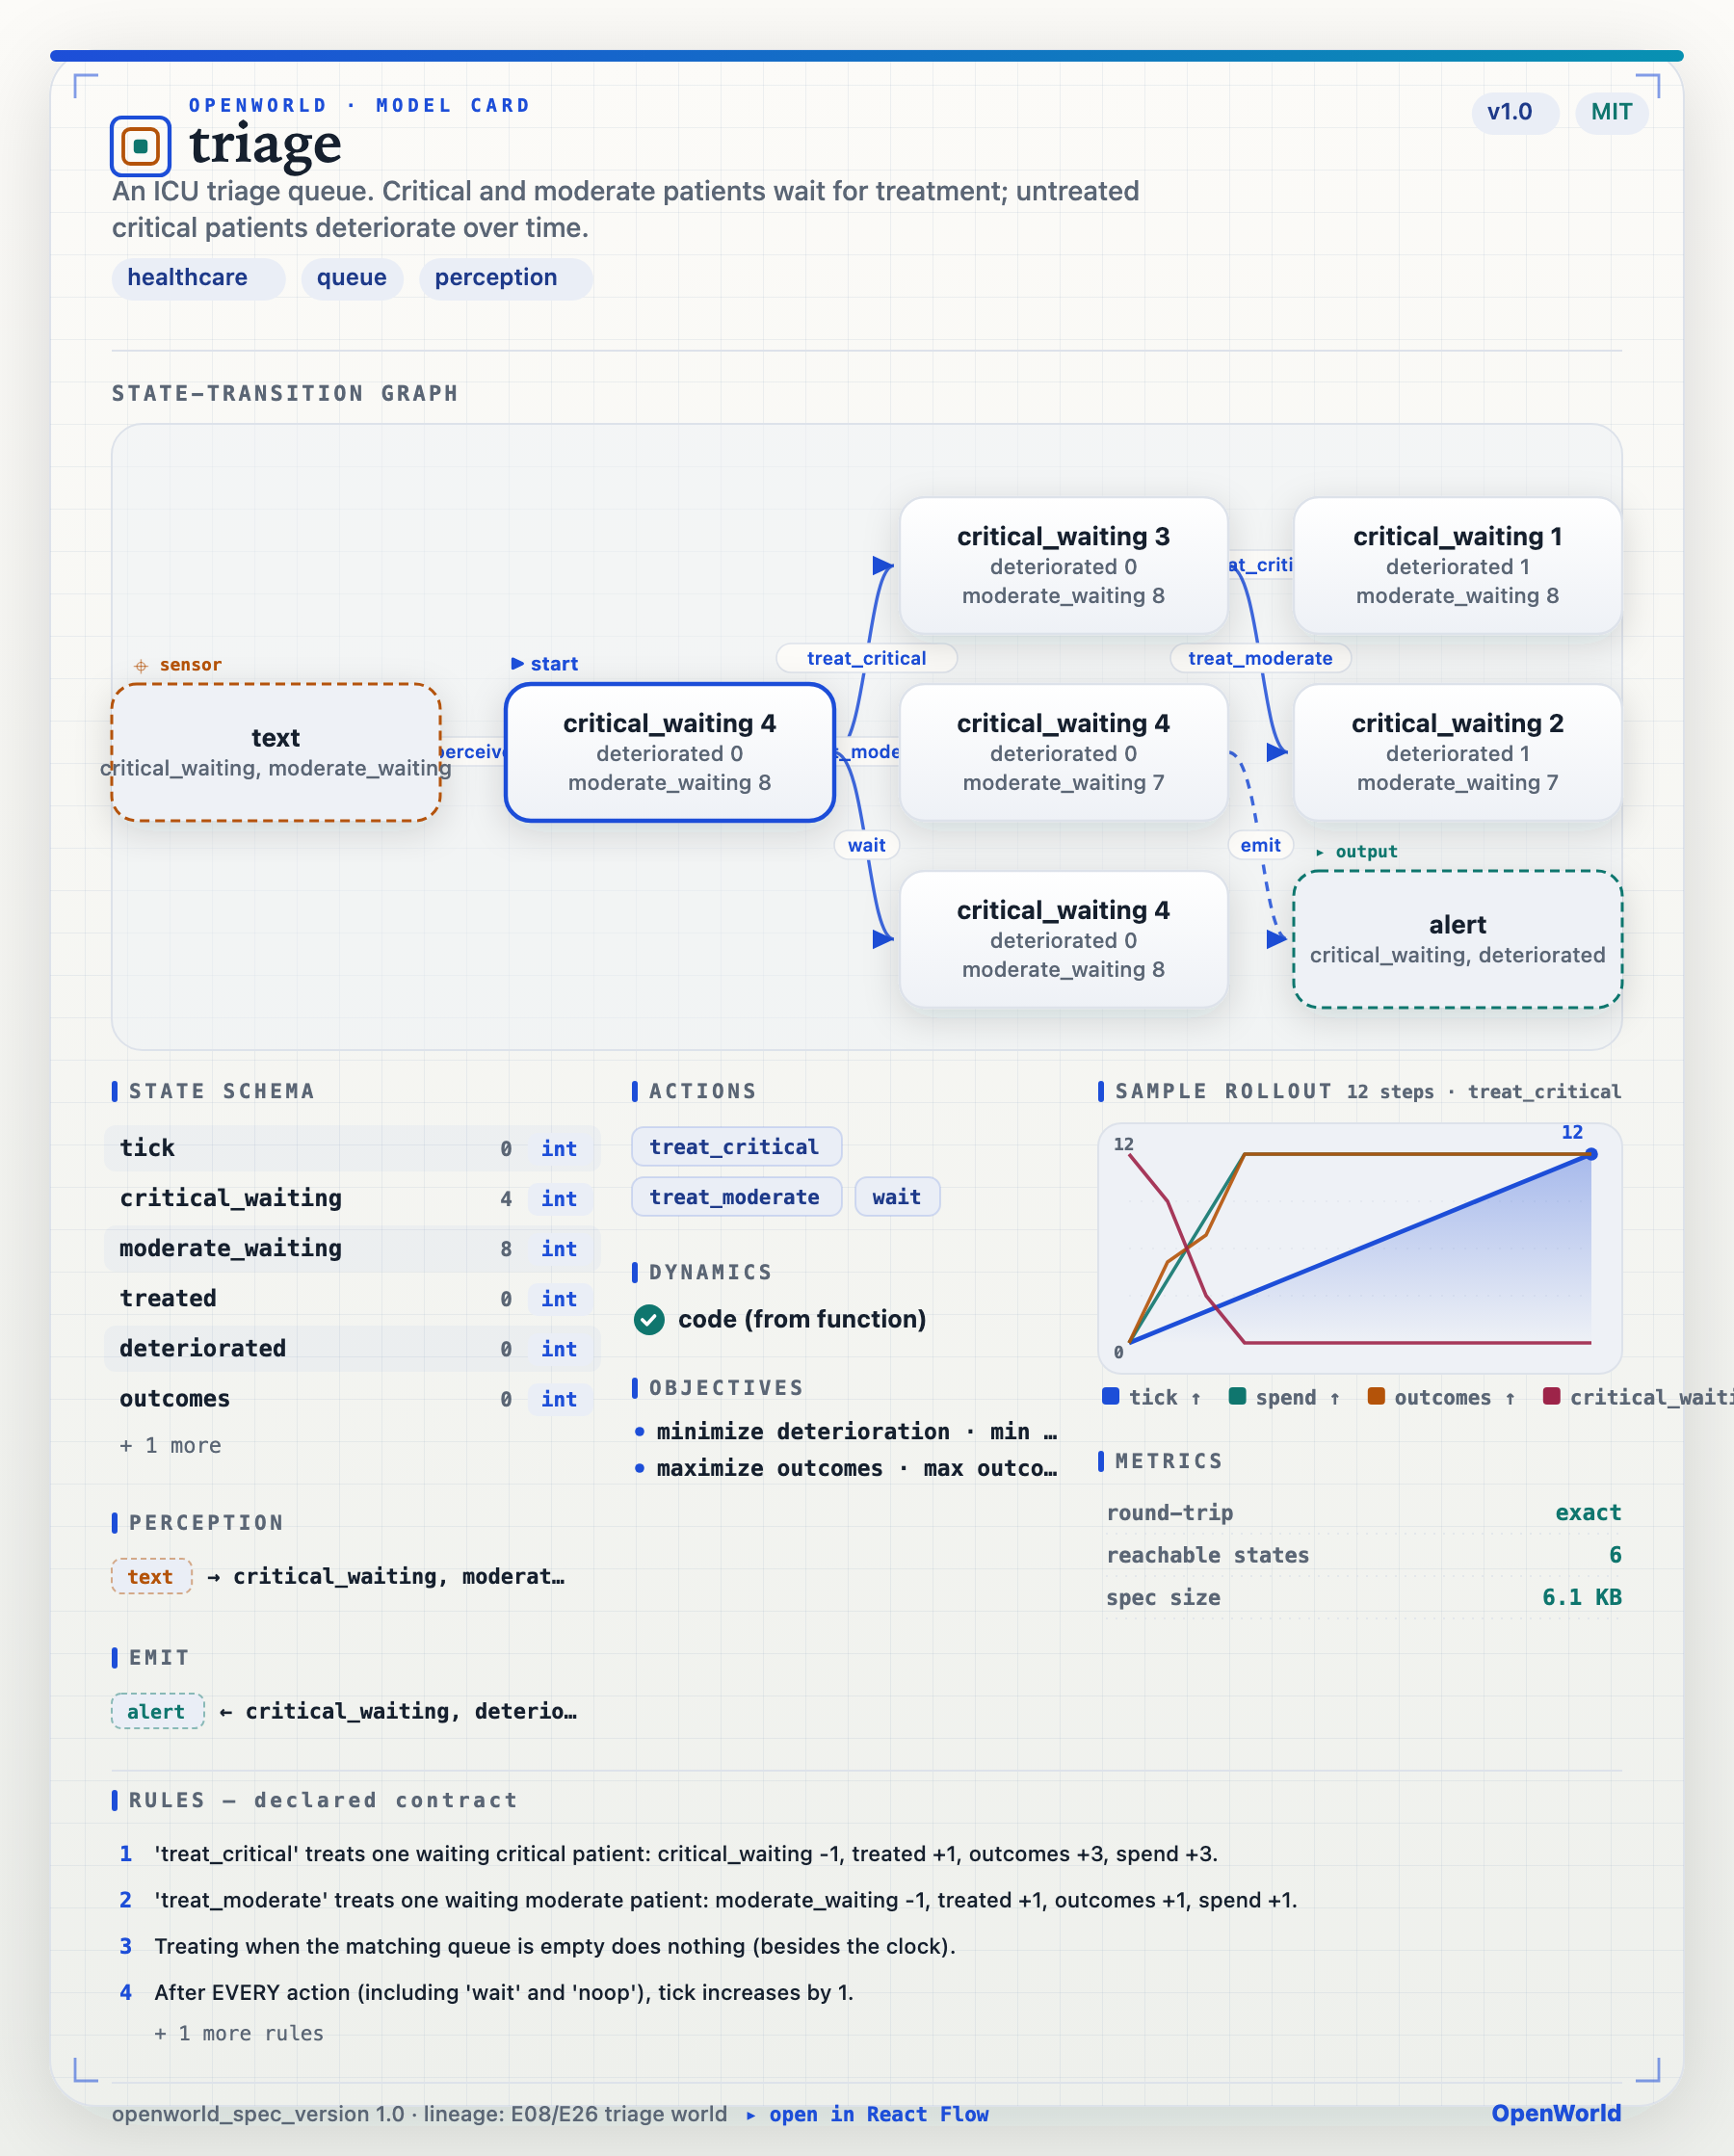
\includegraphics[width=\linewidth,height=0.48\textheight,keepaspectratio]{world_card.png}\vskip3pt{\color{owmuted}\footnotesize One self-contained SVG rendered from a world's spec; round-trips losslessly\par}
\flushleft \vskip3pt{\footnotesize \begin{itemize}
  \item State, rules, dynamics, perception/emit, objectives -- all captured
  \item Exports to Mermaid and React Flow; a marketplace unit for worlds
\end{itemize}}
\end{frame}
\begin{frame}[plain]\centering\vfill
{\color{owochre}\rule{40pt}{2.5pt}}\par\vskip10pt
{\color{owdeep}\bfseries\Large The arc, and what's next\par}\vfill\end{frame}
\begin{frame}{Three ways to use a verified world model}
\begin{itemize}
  \item Tool: serve, plan, verify -- exact, auditable, no training
  \item Per-world test-time training: distill one world's trajectories
  \item World-time compute: traverse a family, generalize to new worlds
  \item Hybrid: generate exact data, internalize it, exact backstop on demand
\end{itemize}
\end{frame}
\begin{frame}{The transferable lessons}
\begin{itemize}
  \item Verified code is bit-exact where learned dynamics compound error
  \item Composition defeats the complexity cliff -- the boundary is measured
  \item Interactive wins are ordered procedures; aim at procedure discovery
  \item Traversing many verified worlds lifts generalization to held-out worlds
\end{itemize}
\end{frame}
\begin{frame}{Limitations and scope}
\begin{itemize}
  \item Scope: symbolic-state worlds; pixel-native remains learned territory
  \item Monolithic synthesis unreliable past \textasciitilde{}8 coupled rules (use composition)
  \item ARC-AGI-3 result is best-of-N and contamination-unmeasured (stated openly)
  \item Next: compositional synthesis, perception-to-symbol, live-protocol evaluation
\end{itemize}
\end{frame}
\begin{frame}[plain]\centering\vfill
{\color{owdeep}\bfseries\LARGE Build the world as verified code. Traverse it for experience. Reason the goal. Serve it to anyone.\par}\vfill\end{frame}
\end{document}
